\section{Prediction quality and error structure}\label{sec:section-06}

The recent audit has 1,056 labeled instrument-dates across 48 sessions. Hybrid accuracy is 37.59\%, while prior accuracy is 40.62\%. Hybrid balanced accuracy is 37.24\% and macro F1 is 0.372. The prior's stronger aggregate accuracy does not imply equal recall across classes; the class report makes that tradeoff visible. Log loss also favors the prior in this sample, so there is no probability-quality improvement to hide behind a change in class balance.

\noindent Table~\ref{tab:5} reports consumed recent-audit forecasts; identical mature observations.

\begin{table}[!htbp]\centering\footnotesize\setlength{\tabcolsep}{3pt}\renewcommand{\arraystretch}{1.14}
\caption{Consumed recent-audit forecasts; identical mature observations}\label{tab:5}
\begin{tabular}{@{}>{\raggedright\arraybackslash}p{\dimexpr 0.14286\textwidth-5.143pt\relax}>{\raggedleft\arraybackslash}p{\dimexpr 0.14286\textwidth-5.143pt\relax}>{\raggedleft\arraybackslash}p{\dimexpr 0.14286\textwidth-5.143pt\relax}>{\raggedleft\arraybackslash}p{\dimexpr 0.14286\textwidth-5.143pt\relax}>{\raggedleft\arraybackslash}p{\dimexpr 0.14286\textwidth-5.143pt\relax}>{\raggedleft\arraybackslash}p{\dimexpr 0.14286\textwidth-5.143pt\relax}>{\raggedleft\arraybackslash}p{\dimexpr 0.14286\textwidth-5.143pt\relax}@{}}
\toprule
\textbf{Model} & \textbf{Rows} & \textbf{Accuracy} & \textbf{Balanced} & \textbf{Macro F1} & \textbf{Log loss} & \textbf{Brier} \\
\midrule
linear & 1,056 & 38.35\% & 37.89\% & 0.378 & 1.1291 & 0.6858 \\
tree & 1,056 & 36.93\% & 36.63\% & 0.366 & 1.1679 & 0.7049 \\
raw\_\allowbreak{}mix & 1,056 & 37.59\% & 37.24\% & 0.372 & 1.1171 & 0.6796 \\
hybrid & 1,056 & 37.59\% & 37.24\% & 0.372 & 1.0882 & 0.6594 \\
prior & 1,056 & 40.62\% & 39.26\% & 0.307 & 1.0756 & 0.6540 \\
always\_\allowbreak{}up & 1,056 & 35.89\% & 33.33\% & 0.176 & 17.7142 & 1.2822 \\
\bottomrule\end{tabular}\par\smallskip
\raggedright\textit{Source:} \path{data/research-v2/tables/diag_forecast_summary.csv}.
\end{table}


\noindent Figure~\ref{fig:4} shows audit confusion matrices with class support; row normalization does not create independent observations.

\begin{figure}[htbp]\centering
% Native editable figure; frozen statistics 0d291b4aebf8c524dc6705d872c070feb990e86a1cebbd59a758f400b240c952
\begin{minipage}[t]{.32\linewidth}\centering
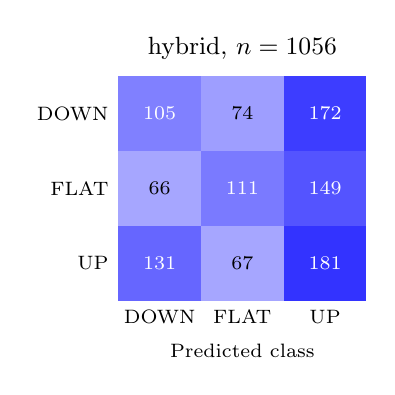
\begin{tikzpicture}[x=1.05cm,y=.95cm,font=\scriptsize]
\fill[blue!50] (0,2) rectangle ++(1,1);\node[text=white] at (0.5,2.5) {105};
\fill[blue!38] (1,2) rectangle ++(1,1);\node[text=black] at (1.5,2.5) {74};
\fill[blue!76] (2,2) rectangle ++(1,1);\node[text=white] at (2.5,2.5) {172};
\fill[blue!35] (0,1) rectangle ++(1,1);\node[text=black] at (0.5,1.5) {66};
\fill[blue!52] (1,1) rectangle ++(1,1);\node[text=white] at (1.5,1.5) {111};
\fill[blue!67] (2,1) rectangle ++(1,1);\node[text=white] at (2.5,1.5) {149};
\fill[blue!60] (0,0) rectangle ++(1,1);\node[text=white] at (0.5,0.5) {131};
\fill[blue!35] (1,0) rectangle ++(1,1);\node[text=black] at (1.5,0.5) {67};
\fill[blue!80] (2,0) rectangle ++(1,1);\node[text=white] at (2.5,0.5) {181};
\node[below] at (0.5,0) {DOWN};\node[left] at (0,2.5) {DOWN};
\node[below] at (1.5,0) {FLAT};\node[left] at (0,1.5) {FLAT};
\node[below] at (2.5,0) {UP};\node[left] at (0,0.5) {UP};
\node[above,font=\small] at (1.5,3.1) {hybrid, $n=1056$};
\node[below] at (1.5,-.45) {Predicted class};\end{tikzpicture}\end{minipage}
\hfill
\begin{minipage}[t]{.32\linewidth}\centering
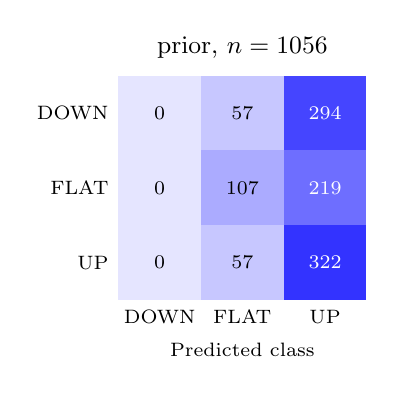
\begin{tikzpicture}[x=1.05cm,y=.95cm,font=\scriptsize]
\fill[blue!10] (0,2) rectangle ++(1,1);\node[text=black] at (0.5,2.5) {0};
\fill[blue!22] (1,2) rectangle ++(1,1);\node[text=black] at (1.5,2.5) {57};
\fill[blue!73] (2,2) rectangle ++(1,1);\node[text=white] at (2.5,2.5) {294};
\fill[blue!10] (0,1) rectangle ++(1,1);\node[text=black] at (0.5,1.5) {0};
\fill[blue!33] (1,1) rectangle ++(1,1);\node[text=black] at (1.5,1.5) {107};
\fill[blue!57] (2,1) rectangle ++(1,1);\node[text=white] at (2.5,1.5) {219};
\fill[blue!10] (0,0) rectangle ++(1,1);\node[text=black] at (0.5,0.5) {0};
\fill[blue!22] (1,0) rectangle ++(1,1);\node[text=black] at (1.5,0.5) {57};
\fill[blue!80] (2,0) rectangle ++(1,1);\node[text=white] at (2.5,0.5) {322};
\node[below] at (0.5,0) {DOWN};\node[left] at (0,2.5) {DOWN};
\node[below] at (1.5,0) {FLAT};\node[left] at (0,1.5) {FLAT};
\node[below] at (2.5,0) {UP};\node[left] at (0,0.5) {UP};
\node[above,font=\small] at (1.5,3.1) {prior, $n=1056$};
\node[below] at (1.5,-.45) {Predicted class};\end{tikzpicture}\end{minipage}
\hfill
\begin{minipage}[t]{.32\linewidth}\centering
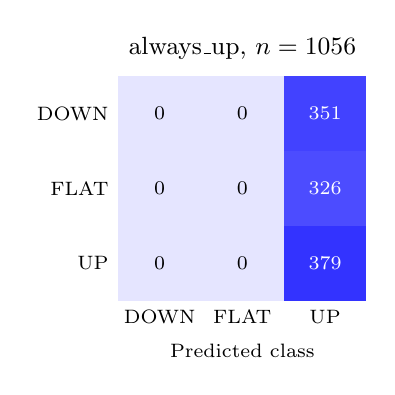
\begin{tikzpicture}[x=1.05cm,y=.95cm,font=\scriptsize]
\fill[blue!10] (0,2) rectangle ++(1,1);\node[text=black] at (0.5,2.5) {0};
\fill[blue!10] (1,2) rectangle ++(1,1);\node[text=black] at (1.5,2.5) {0};
\fill[blue!74] (2,2) rectangle ++(1,1);\node[text=white] at (2.5,2.5) {351};
\fill[blue!10] (0,1) rectangle ++(1,1);\node[text=black] at (0.5,1.5) {0};
\fill[blue!10] (1,1) rectangle ++(1,1);\node[text=black] at (1.5,1.5) {0};
\fill[blue!70] (2,1) rectangle ++(1,1);\node[text=white] at (2.5,1.5) {326};
\fill[blue!10] (0,0) rectangle ++(1,1);\node[text=black] at (0.5,0.5) {0};
\fill[blue!10] (1,0) rectangle ++(1,1);\node[text=black] at (1.5,0.5) {0};
\fill[blue!80] (2,0) rectangle ++(1,1);\node[text=white] at (2.5,0.5) {379};
\node[below] at (0.5,0) {DOWN};\node[left] at (0,2.5) {DOWN};
\node[below] at (1.5,0) {FLAT};\node[left] at (0,1.5) {FLAT};
\node[below] at (2.5,0) {UP};\node[left] at (0,0.5) {UP};
\node[above,font=\small] at (1.5,3.1) {always\_up, $n=1056$};
\node[below] at (1.5,-.45) {Predicted class};\end{tikzpicture}\end{minipage}
\caption{Audit confusion matrices with class support; row normalization does not create independent observations.}\label{fig:4}
\end{figure}

\noindent Table~\ref{tab:6} reports audit class report for calibrated mixture and prior.

\begin{table}[!htbp]\centering\footnotesize\setlength{\tabcolsep}{3pt}\renewcommand{\arraystretch}{1.14}
\caption{Audit class report for calibrated mixture and prior}\label{tab:6}
\begin{tabular}{@{}>{\raggedright\arraybackslash}p{\dimexpr 0.16667\textwidth-5.000pt\relax}>{\raggedright\arraybackslash}p{\dimexpr 0.16667\textwidth-5.000pt\relax}>{\raggedleft\arraybackslash}p{\dimexpr 0.16667\textwidth-5.000pt\relax}>{\raggedleft\arraybackslash}p{\dimexpr 0.16667\textwidth-5.000pt\relax}>{\raggedleft\arraybackslash}p{\dimexpr 0.16667\textwidth-5.000pt\relax}>{\raggedleft\arraybackslash}p{\dimexpr 0.16667\textwidth-5.000pt\relax}@{}}
\toprule
\textbf{Model} & \textbf{Class} & \textbf{Precision} & \textbf{Recall} & \textbf{F1} & \textbf{Support} \\
\midrule
hybrid & DOWN & 0.348 & 0.299 & 0.322 & 351 \\
hybrid & FLAT & 0.440 & 0.340 & 0.384 & 326 \\
hybrid & UP & 0.361 & 0.478 & 0.411 & 379 \\
prior & DOWN & 0.000 & 0.000 & 0.000 & 351 \\
prior & FLAT & 0.484 & 0.328 & 0.391 & 326 \\
prior & UP & 0.386 & 0.850 & 0.530 & 379 \\
\bottomrule\end{tabular}\par\smallskip
\raggedright\textit{Source:} \path{data/research-v2/tables/diag_class_report.csv}.
\end{table}


Per-class reporting prevents a common majority class from concealing weak recall elsewhere. Precision asks what fraction of a model's class assignments were right; recall asks how many observed examples of that class it recovered. F1 combines these two rates, and support states the denominator. Row-normalized confusion matrices emphasize which true classes are confused, while raw counts identify where most mistakes occur. The dominant transition can change when class prevalence changes even if the conditional error rates remain stable.

The most frequent off-diagonal transition in the audit is DOWN to UP, with 172 errors, or 49.00\% of that true class. Temperature scaling changes raw-mixture log loss by -0.0289 with interval [-0.0476, -0.0065]. The argmax labels are unchanged, as expected for positive temperature scaling. Better calibrated confidence can coexist with unchanged directional accuracy and still fail to beat the prior.

\noindent Figure~\ref{fig:5} shows probability reliability and confidence coverage, including bin support and uncertainty.

\begin{figure}[htbp]\centering
% Native editable figure; frozen statistics 0d291b4aebf8c524dc6705d872c070feb990e86a1cebbd59a758f400b240c952
\begin{minipage}[t]{.48\linewidth}\centering
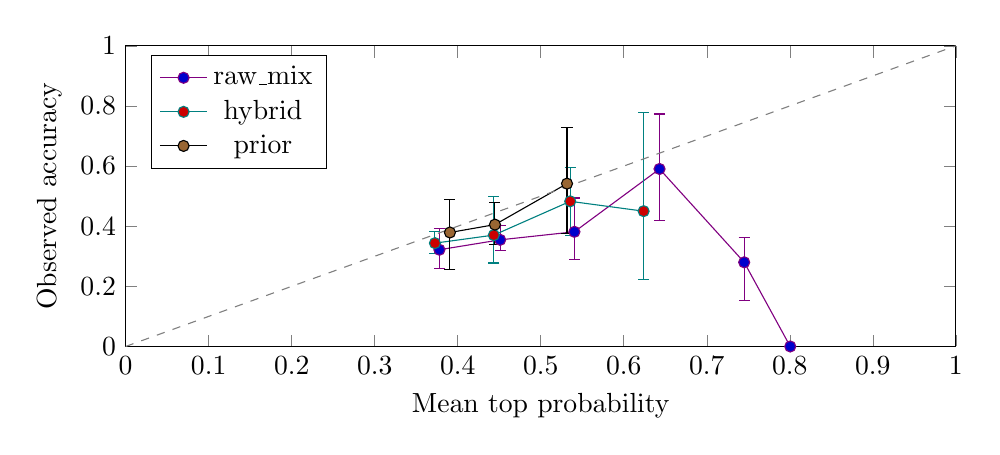
\begin{tikzpicture}
\begin{axis}[width=\linewidth,height=5.4cm,xmin=0,xmax=1,ymin=0,ymax=1,xlabel={Mean top probability},ylabel={Observed accuracy},legend pos=north west]
\addplot+[violet,mark=*,error bars/.cd,y dir=both,y explicit] table[x=x,y=y,y error minus=lo,y error plus=hi,row sep=\\]{x y lo hi\\0.377941396125 0.321739130435 0.061465157832 0.0711180124224\\
0.451112648618 0.354709418838 0.036937544687 0.0473755946032\\
0.540554545882 0.381381381381 0.0908637745748 0.112484584502\\
0.643079026906 0.590361445783 0.171317044239 0.182983792312\\
0.745038302803 0.28 0.12625 0.0836363636364\\
0.800526928081 0 0 0\\};
\addlegendentry{raw\_mix}
\addplot+[teal,mark=*,error bars/.cd,y dir=both,y explicit] table[x=x,y=y,y error minus=lo,y error plus=hi,row sep=\\]{x y lo hi\\0.372554098696 0.343680709534 0.033947623608 0.0388077697283\\
0.443490294143 0.370454545455 0.0928049251844 0.127299994627\\
0.535517133114 0.48275862069 0.113193403298 0.113135192247\\
0.62391873958 0.45 0.227777777778 0.327777777778\\};
\addlegendentry{hybrid}
\addplot+[black,mark=*,error bars/.cd,y dir=both,y explicit] table[x=x,y=y,y error minus=lo,y error plus=hi,row sep=\\]{x y lo hi\\0.390609751495 0.379146919431 0.123131687251 0.11015361194\\
0.444825090677 0.405269761606 0.0664880431194 0.0743930239297\\
0.531641069397 0.541666666667 0.166666666667 0.1875\\};
\addlegendentry{prior}
\addplot+[gray,mark=none,dashed] coordinates {(0,0) (1,1)};

\end{axis}
\end{tikzpicture}
\end{minipage}
\hfill
\begin{minipage}[t]{.48\linewidth}\centering
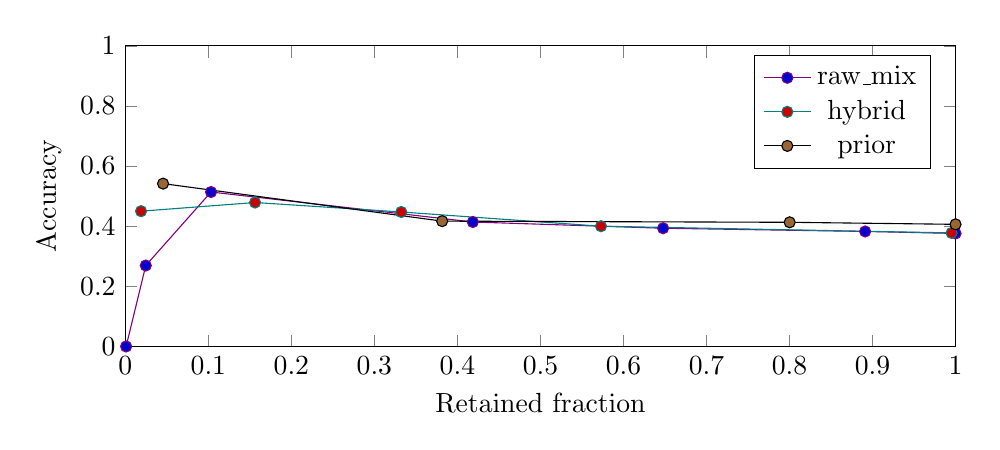
\begin{tikzpicture}
\begin{axis}[width=\linewidth,height=5.4cm,xmin=0,xmax=1,ymin=0,ymax=1,xlabel={Retained fraction},ylabel={Accuracy},legend pos=north east]
\addplot+[violet,mark=none,mark=*] coordinates {(1,0.375946969697) (0.891098484848,0.3825717322) (0.647727272727,0.393274853801) (0.418560606061,0.414027149321) (0.10321969697,0.51376146789) (0.0246212121212,0.269230769231) (0.00094696969697,0)};
\addlegendentry{raw\_mix}
\addplot+[teal,mark=none,mark=*] coordinates {(0.995265151515,0.37773549001) (0.572916666667,0.4) (0.332386363636,0.447293447293) (0.15625,0.478787878788) (0.0189393939394,0.45)};
\addlegendentry{hybrid}
\addplot+[black,mark=none,mark=*] coordinates {(1,0.40625) (0.800189393939,0.413017751479) (0.381628787879,0.416873449132) (0.0454545454545,0.541666666667)};
\addlegendentry{prior}

\end{axis}
\end{tikzpicture}
\end{minipage}
\caption{Probability reliability and confidence coverage, including bin support and uncertainty.}\label{fig:5}
\end{figure}

\noindent Table~\ref{tab:7} reports audit mixture confidence coverage; thresholds fixed for description.

\begin{table}[!htbp]\centering\footnotesize\setlength{\tabcolsep}{3pt}\renewcommand{\arraystretch}{1.14}
\caption{Audit mixture confidence coverage; thresholds fixed for description}\label{tab:7}
\begin{tabular}{@{}>{\raggedleft\arraybackslash}p{\dimexpr 0.20000\textwidth-4.800pt\relax}>{\raggedleft\arraybackslash}p{\dimexpr 0.20000\textwidth-4.800pt\relax}>{\raggedleft\arraybackslash}p{\dimexpr 0.20000\textwidth-4.800pt\relax}>{\raggedleft\arraybackslash}p{\dimexpr 0.20000\textwidth-4.800pt\relax}>{\raggedleft\arraybackslash}p{\dimexpr 0.20000\textwidth-4.800pt\relax}@{}}
\toprule
\textbf{Threshold} & \textbf{Retained} & \textbf{Dates} & \textbf{Coverage} & \textbf{Accuracy} \\
\midrule
0.34 & 1,051 & 48 & 99.53\% & 37.77\% \\
0.40 & 605 & 48 & 57.29\% & 40.00\% \\
0.45 & 351 & 48 & 33.24\% & 44.73\% \\
0.50 & 165 & 48 & 15.62\% & 47.88\% \\
0.60 & 20 & 15 & 1.89\% & 45.00\% \\
0.70 & 0 & 0 & 0.00\% & - \\
0.80 & 0 & 0 & 0.00\% & - \\
0.90 & 0 & 0 & 0.00\% & - \\
\bottomrule\end{tabular}\par\smallskip
\raggedright\textit{Source:} \path{data/research-v2/tables/diag_coverage.csv}.
\end{table}


Confidence-coverage curves retain only predictions above fixed confidence cutoffs and report both accuracy and remaining observations. A higher accuracy at low coverage can be practically irrelevant when almost no decisions remain. These curves are diagnostics, not an opportunity to choose the best threshold after viewing outcomes. Reliability-bin uncertainty is also limited by correlated dates; bins with little support cannot justify a confident calibration claim. For trading, an apparently well-calibrated probability still needs useful class-return estimates and enough expected advantage to pay costs.

\noindent Figure~\ref{fig:6} shows paired audit forecast effects and date-block uncertainty. Lower log loss is better.

\begin{figure}[htbp]\centering
% Native editable figure; frozen statistics 0d291b4aebf8c524dc6705d872c070feb990e86a1cebbd59a758f400b240c952
\begin{minipage}[t]{.32\linewidth}\centering
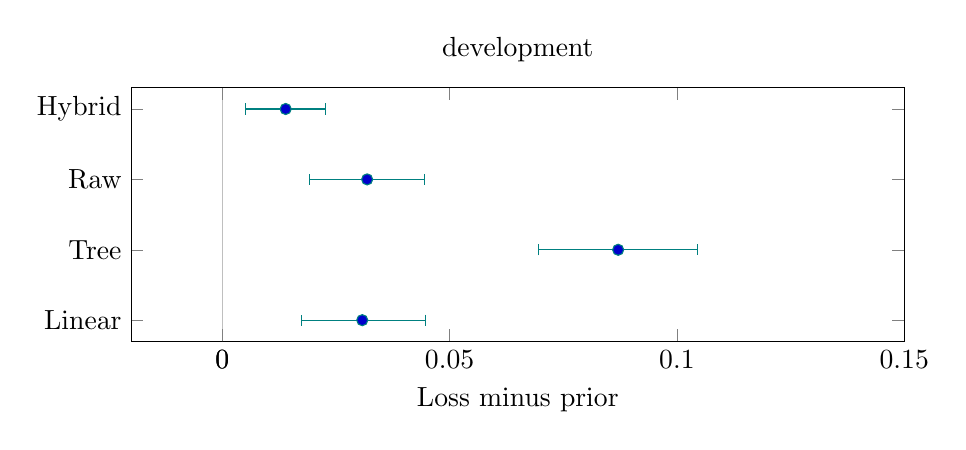
\begin{tikzpicture}
\begin{axis}[width=.94\linewidth,height=4.8cm,title={development},ytick={0,1,2,3},yticklabels={Linear,Tree,Raw,Hybrid},xlabel={Loss minus prior},xmin=-.02,xmax=.15,xtick={0,.05,.10,.15},scaled x ticks=false,x tick label style={/pgf/number format/fixed,/pgf/number format/precision=2},extra x ticks={0},extra x tick style={grid=major}]
\addplot+[teal,only marks,mark=*,error bars/.cd,x dir=both,x explicit] table[x=x,y=y,x error minus=lo,x error plus=hi,row sep=\\]{x y lo hi\\0.0307945818317 0 0.0133978723424 0.0138576511937\\
0.0870756476825 1 0.0175279184931 0.0174131845911\\
0.0318687091039 2 0.0126557943824 0.0125213618115\\
0.013947459402 3 0.00878659866028 0.00885623096892\\};

\end{axis}
\end{tikzpicture}
\end{minipage}
\hfill
\begin{minipage}[t]{.32\linewidth}\centering
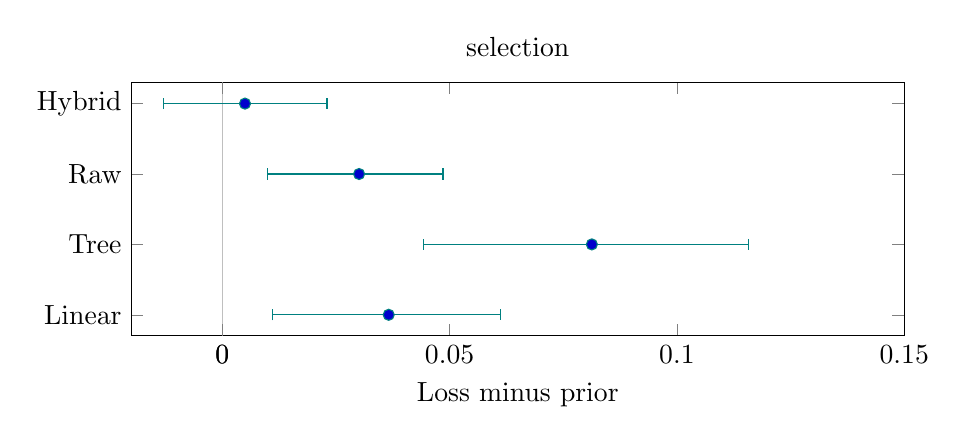
\begin{tikzpicture}
\begin{axis}[width=.94\linewidth,height=4.8cm,title={selection},ytick={0,1,2,3},yticklabels={Linear,Tree,Raw,Hybrid},xlabel={Loss minus prior},xmin=-.02,xmax=.15,xtick={0,.05,.10,.15},scaled x ticks=false,x tick label style={/pgf/number format/fixed,/pgf/number format/precision=2},extra x ticks={0},extra x tick style={grid=major}]
\addplot+[teal,only marks,mark=*,error bars/.cd,x dir=both,x explicit] table[x=x,y=y,x error minus=lo,x error plus=hi,row sep=\\]{x y lo hi\\0.0366086965343 0 0.0255516950915 0.0246095487994\\
0.0812901260331 1 0.0371062104379 0.0344655441593\\
0.030095155111 2 0.0201815717422 0.0184559397131\\
0.0050018252014 3 0.0178401338044 0.0180481599458\\};

\end{axis}
\end{tikzpicture}
\end{minipage}
\hfill
\begin{minipage}[t]{.32\linewidth}\centering
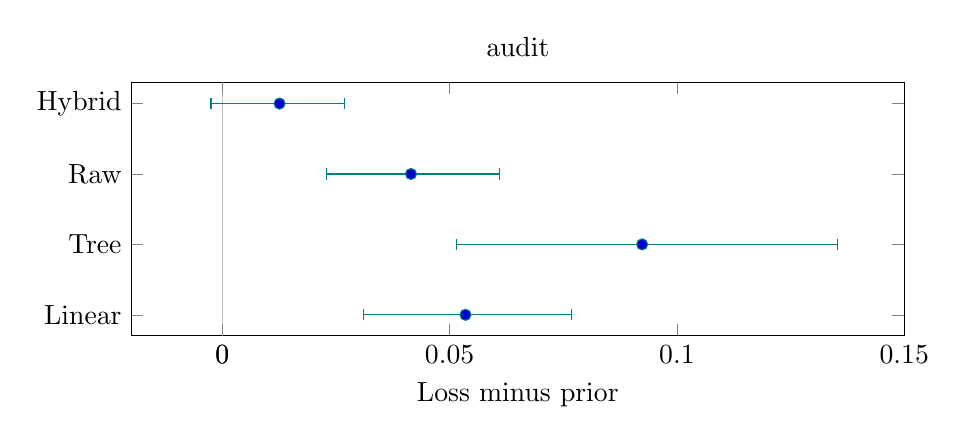
\begin{tikzpicture}
\begin{axis}[width=.94\linewidth,height=4.8cm,title={audit},ytick={0,1,2,3},yticklabels={Linear,Tree,Raw,Hybrid},xlabel={Loss minus prior},xmin=-.02,xmax=.15,xtick={0,.05,.10,.15},scaled x ticks=false,x tick label style={/pgf/number format/fixed,/pgf/number format/precision=2},extra x ticks={0},extra x tick style={grid=major}]
\addplot+[teal,only marks,mark=*,error bars/.cd,x dir=both,x explicit] table[x=x,y=y,x error minus=lo,x error plus=hi,row sep=\\]{x y lo hi\\0.0534971109377 0 0.0225075059482 0.0232500211536\\
0.0923489707796 1 0.0408988275295 0.0429054660783\\
0.0415131268524 2 0.0186156550241 0.0193978388432\\
0.0126044345825 3 0.0150693518368 0.0143454615776\\};

\end{axis}
\end{tikzpicture}
\end{minipage}
\caption{Paired audit forecast effects and date-block uncertainty. Lower log loss is better.}\label{fig:6}
\end{figure}

For the primary audit hybrid-minus-prior comparison, the estimated loss difference is 0.0126, the bootstrap standard error is 0.0076, and the approximate 80\%-power detectable magnitude is 0.0213. With 48 dates and primary blocks of 10 dates, the effective information is much smaller than the number of stock rows suggests. This approximation ignores additional uncertainty about structural change and is not a prospective power guarantee.
